\documentclass[graphics]{beamer}
\usepackage{xcolor}
\usepackage{graphicx}
\usepackage{verbatim}
\usepackage{wrapfig}
\useoutertheme{shadow}
%\usecolortheme{orchid}
\usecolortheme{seahorse}


% math commands
\newcommand{\be}{\begin{eqnarray}}
\newcommand{\ee}{\end{eqnarray}}
\newcommand{\beq}{\begin{equation}}
\newcommand{\eeq}{\end{equation}}
\def\simless{\mathbin{\lower 3pt\hbox
      {$\rlap{\raise 5pt\hbox{$\char'074$}}\mathchar"7218$}}}
\def\simgreat{\mathbin{\lower 3pt\hbox
      {$\rlap{\raise 5pt\hbox{$\char'076$}}\mathchar"7218$}}} %> or of order

% variables

\def\toonscale{0.45}
\def\mboxy#1{\mbox{\small #1}}

\defbeamertemplate*{title page}{customized}[1][]
{
  \usebeamerfont{title}\inserttitle\par
  \usebeamerfont{subtitle}\usebeamercolor[fg]{subtitle}\insertsubtitle\par
  \bigskip
  \usebeamerfont{author}\insertauthor\par
  \usebeamerfont{institute}\insertinstitute\par
  \usebeamerfont{date}\insertdate\par
  \usebeamercolor[fg]{titlegraphic}\inserttitlegraphic
}
\begin{comment}
\AtBeginSection[]{
  \frame{
    \frametitle{Outline}
    \tableofcontents[currentsection]
  }
}
\end{comment}


\title{Interstellar Lenses}
%\subtitle{}
\author[U. Pen]{{
\textcolor{green}{\small Dana Simard, Robert Main, Daniel Baker}, 
\textcolor{cyan}{\small I-Sheng Yang, Franz Kirsten} 
\textcolor{darkgray}{\small U. Pen, M. van Kerkwijk, K. Vanderlinde, J-P Macquart and many more}
}
\\[8mm] 
}
\date{September 19, 2016}


\begin{document}

\frame{
\vspace{-0.5in}
\begin{center}  
%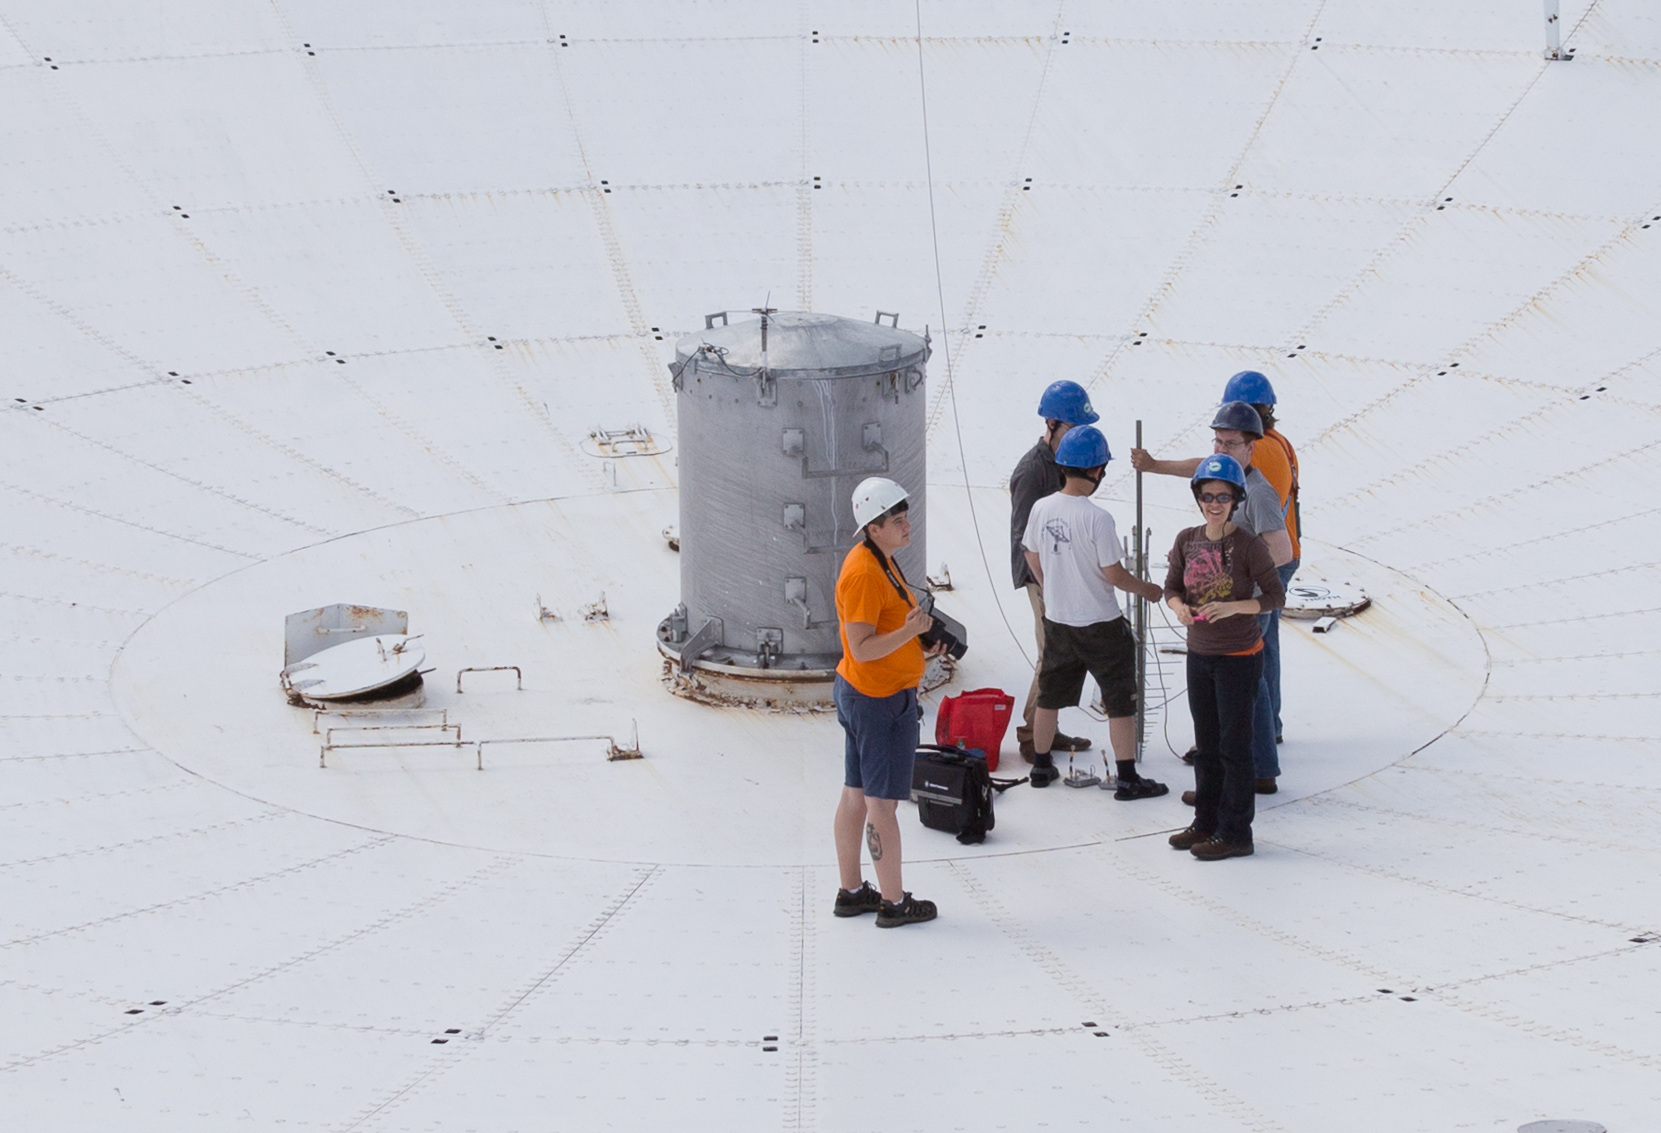
\includegraphics[width=4.4in]{Figures/IMG-0438-by-Andre-cropped.jpg}
\end{center}
\begin{picture}(320,250)
\put(-50,60){
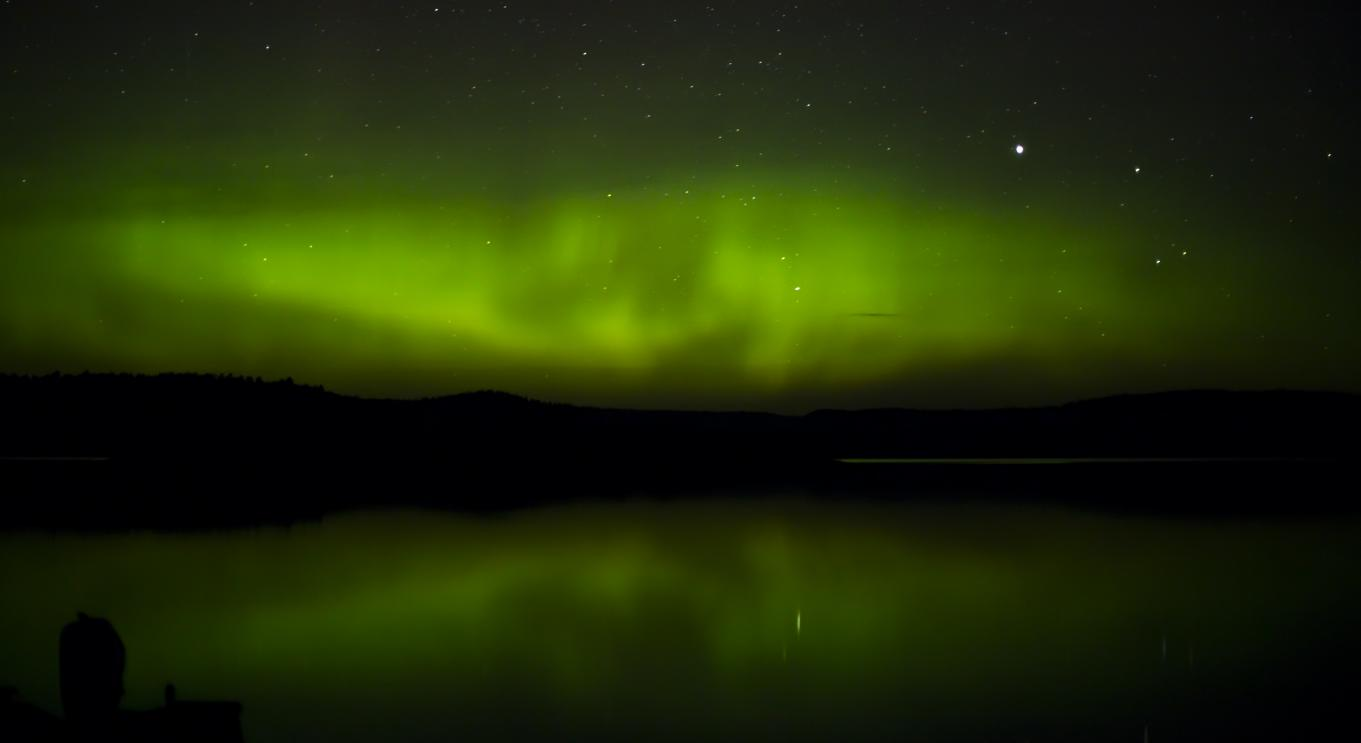
\includegraphics[width=5.5in]{Figures/traverse-aurora.jpg}}
\end{picture}
\vspace{-4in}
\\
image credit: Andre Recnik
\\
\vspace{1in}
\titlepage
}

%\section*{Introduction}
\section{Introduction}

\begin{comment}
  \subsection{Outline}

  \frame{
    \frametitle{Outline}
    \tableofcontents
  }
\end{comment}


\section{Lensing}

\frame{
    \frametitle{Facts}
    \begin{itemize}
      \item multipath propagation leads to delays $\sim$ ms
      \item bending angles $\theta\sim$ mas
      \item for diffraction $\theta \sim \lambda/D \implies D \sim 1000$km
      \item for refraction $\theta \sim \Delta n \implies n_e \sim 100$cm$^{-3}$
        \item observed dominant isolated 1-D scattering screens
          (Stinebring et al 2000++: inverted parabolic arcs, Brisken et al:
          2010 VLBI)
    \end{itemize}

}

  \frame{
    \frametitle{Sheets}
\center{
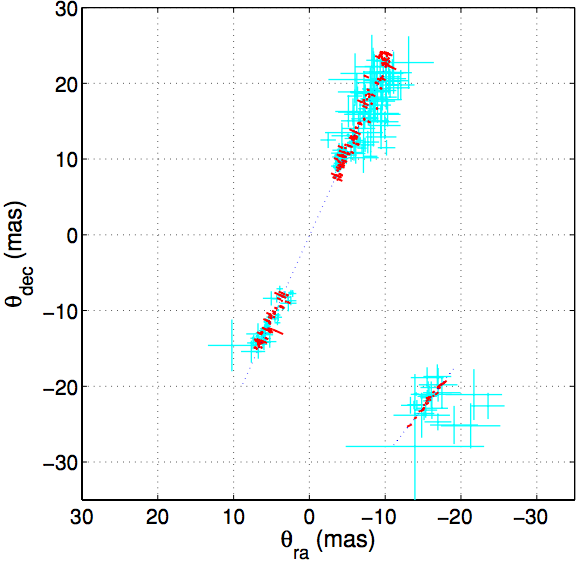
\includegraphics[width=2.9in]{Figures/brisken.png}
}
\vspace{-1.5in} 

\hspace{-4in} $D_S=640$pc

\hspace{-4in} $D_L=400$pc

\hspace{-3.6in} Brisken et al 2010

\vspace{1in}
}

\frame{
    \frametitle{Refraction}
    \begin{itemize}
      \item to form real image for two light rays separated by $D\sim 10^{10}$m
        requires $\sim\lambda$ path length difference.
      \item $\lambda=\int_z \Delta n \implies \Delta n \sim  \lambda/z$ 
      \item for isotropic lens $z\sim D$ we get
      \item $\Delta n=-\lambda^2r_en_e/2\pi \sim  10^{-11}\frac{n_e}{0.03 \rm cm^{-3}}
        (\frac{\lambda}{\rm m})^2$
        \item at face value requires $n_e \gg 1$ (free electrons, $T>$10,000K)!
    \end{itemize}

}

\frame{
    \frametitle{Challenges to refactive picture}
    \begin{itemize}
      \item unreasonable plasma densities for pressure equilibrium $P=nkT$
      \item proposed solutions: 1. explosive. strange quarklets (P\'erez-Garc\'ia et
        al), baryonic dark matter (Walker)
        \item 2. static. isotropic: cosmic strings
        (Thompson), 
      \item anisotropic: folded sheets (Goldreich-Shridhar 2006,
        ULP-Levin 2014)
      \item Note: random filaments not dominated by extreme
        alignments, sheets always dominated by extreme.
    \end{itemize}
}


\frame{
    \frametitle{Diffraction}
    \begin{itemize}
      \item first proposed half a century ago
      \item thought due to turbulence on scales $D\sim 1000$km
      \item angles depend only on length scale, image intensity depends on
        density contrast
      \item intensity ok if space filling
      \item hard to reconcile with inverted parabolic arclets, VLBI
    \end{itemize}
}




  \frame{
    \frametitle{Speculation}
    \begin{itemize}
      \item reconnection sheets
    \item grazing incidence
    \item ULP + King 2012
    \item ULP + Levin 2014
    \item Liu + ULP 2015
    \item 1-D structure
    \item localized scattering
%    \item predicts RM gradient
    \end{itemize}
\begin{picture}(320,235)
\put(110,170){
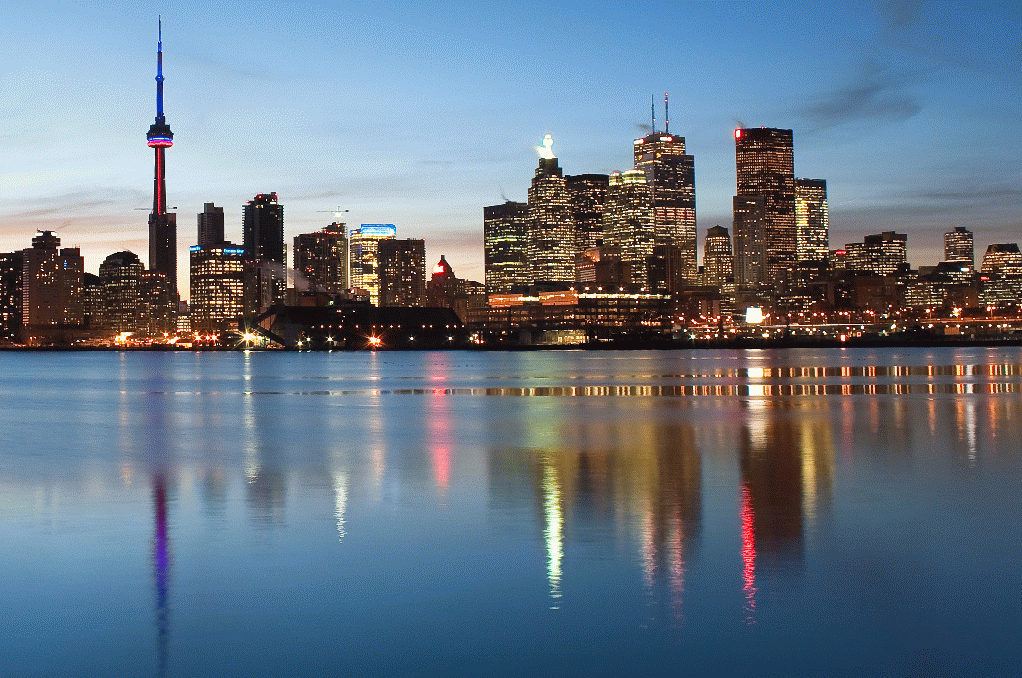
\includegraphics[width=3.0in]{Figures/toronto-skyline.png}}
\put(-60,-207){
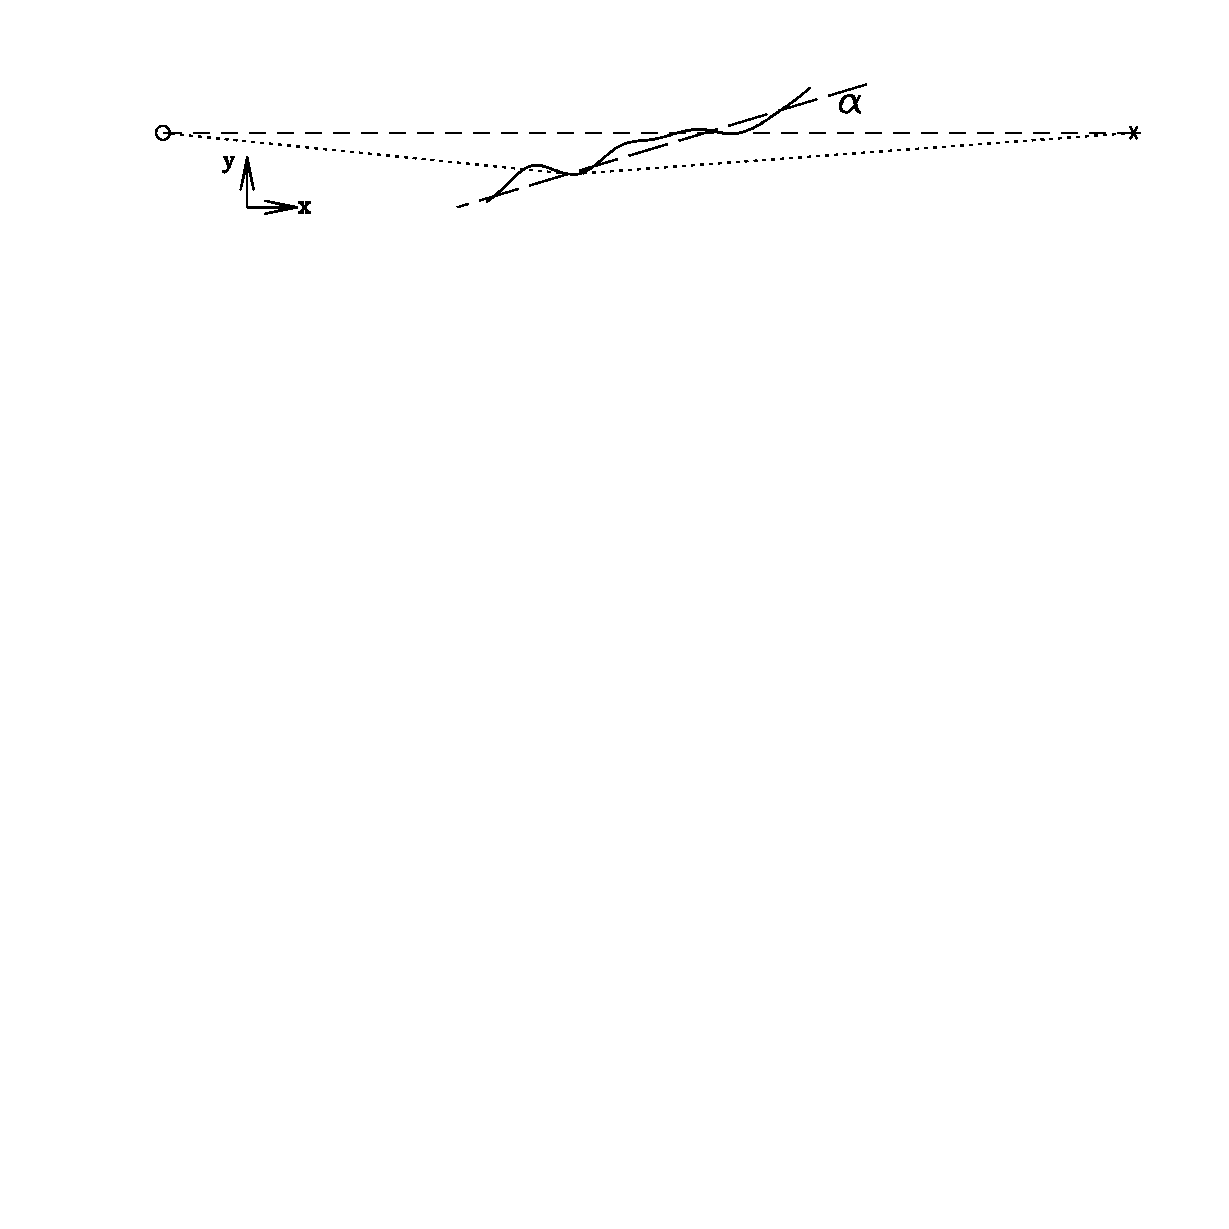
\includegraphics[width=5.5in]{Figures/sheetgeom.eps}}
\end{picture}
  }
  \frame{
    \frametitle{Folds}
\begin{center}
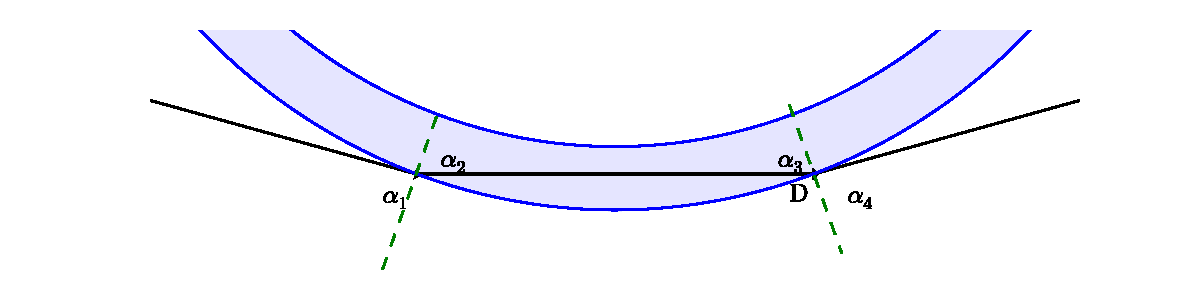
\includegraphics[width=3.9in]{Figures/refraction.pdf}
\end{center}

Refraction of light rays near point D.  The black lines
  are the light paths.  The shaded region indicates the lensing sheet
  caustic.  The angles obey Snell's Law
  $\frac{\sin(\alpha_1)}{\sin(\alpha_2)}=\frac{\sin(\alpha_4)}{\sin(\alpha_3)}=\frac{n_{\rm sheet}}{n_{\rm
    ISM}.$ }
}

  \frame{
    \frametitle{Magnetized plasmas}
    \begin{itemize}
      \item local fields relax to straight lines: anlogy to
        ferromagnet (Gruzinov 2009, braithwaite 2015)
      \item domain boundaries form with current sheets
      \item likely long lived (Sweet-Parker 1956)
      \item corrugated by 'ducted waves'
      \item not to be confused by 'tearing modes' etc.
    \end{itemize}
  }



  \frame{
    \frametitle{Predictions}
    \begin{itemize}
      \item doppler velocity dependence of RM (LOFAR?)
      \item (non-) evolution of inverted arclets, VLBI image positions
      \item (evolution of) space-VLBI visibilities
      \item multi-plane geometries (Liu+Pen 2015)
    \end{itemize}
  }


  \frame{
    \frametitle{Looking Forward}
    \begin{itemize}
      \item new paradigm emerging for ISM structure
      \item pulsar VLBI monitoring
        \item connection to Extreme Scattering Events (ESE).
      \item galactic center scattering
      \item magnetosphere mapping
      \item see talks by Dana, Rob, Daniel, Franz, etc
    \end{itemize}
  }

\end{document}
